% =====================================================================
%  §2. Модель Бланко: эквивалентная схема решётки проводов
%
%  ЖАНР (STYLE.md): учебная литература. Ни путей, ни имён программ, ни
%  номеров гипотез. Прослеживаемость — ключи \srckey{2.x} и приложение.
%
%  Содержательная основа: Blanco A., Fonti S., Piacente A. Transmission
%  coefficients of free-standing wire grids in the far infrared: a
%  theoretical approach for easy computation // Infrared Physics. 1986.
%  Vol. 26, no. 6. P. 357-363. DOI 10.1016/0020-0891(86)90058-8
%  (библиографическая сверка выполнена другой сессией, ключ 2.1).
% =====================================================================
\section{Модель Бланко: эквивалентная схема решётки проводов}
\label{sec:blanco}
\markboth{§\thesection. Модель Бланко}{}

В §\ref{sec:electrodynamics} решётка проводов была принята как данность: сплошной анизотропный
лист, задаваемый двумя комплексными числами $\tperp(\nu)$, $\tpar(\nu)$ на каждой частоте. В
§\ref{sec:jones} эти два числа заняли своё место в матрице элемента и дали угловую зависимость
$U(\theta)$. Оставался открытым главный вопрос: \emph{откуда берутся сами $\tperp$ и $\tpar$}, если
считать не эффективный лист, а настоящую решётку из круглых проводов с диаметром~$D$ и
периодом~$P$? Ответ~--- предмет этого параграфа, и он же задаёт первую жёсткую границу
применимости, с которой предстоит работать всему дальнейшему изложению.

\begin{tcolorbox}[enhanced,colback=cPanel,colframe=cGrid,boxrule=0.8pt,arc=2pt,
                  title={\bfseries\color{cAccent} Пререквизиты},coltitle=cAccent,
                  attach boxed title to top left={xshift=6pt,yshift=-2pt},
                  boxed title style={colback=cPanel,boxrule=0pt,arc=0pt},top=10pt]
\textbf{Нужно знать:} §\ref{sec:electrodynamics} (подволновой режим $P/\lambda\lesssim0{,}2$,
эванесцентность высших дифракционных порядков, параметр плотности $D/P$); понятие комплексного
сопротивления (импеданса) двухполюсника; последовательное и параллельное соединение элементов
цепи.\\[0.3em]
\textbf{Знать НЕ нужно:} строгую теорию дифракции на периодических структурах (ряды
Рэлея--Флоке, интегральные уравнения на профиле провода). Результат этой теории пересказывается
здесь в готовом виде~--- в форме, которую предложили сами авторы модели.
\end{tcolorbox}

% ---------------------------------------------------------------------
\subsection{От дифракционной задачи к электрической цепи}
\label{subsec:circuit-idea}

\begin{intuition}
Строгая электродинамическая задача~--- рассеяние волны на бесконечной решётке проводов~--- в общем
случае очень сложна: нужно решать интегральное уравнение на поверхности каждого провода. Но в
подволновом режиме ($P/\lambda\lesssim0{,}2$, §\ref{sec:electrodynamics}) распространяется только
нулевой дифракционный порядок, а все остальные экспоненциально затухают в первые же доли длины
волны от решётки. Это резко упрощает задачу: решётку можно заменить \emph{чёрным ящиком},
характеризуемым всего двумя числами на входе и выходе~--- ровно так же, как в электротехнике
сложную цепь заменяют одним эквивалентным сопротивлением, если интересует только то, что видно
снаружи.
\end{intuition}

\begin{strict}[: почему замена вообще законна]
Периодическая структура с периодом $P<\lambda$ поддерживает единственную распространяющуюся волну
по обе стороны от решётки~--- саму падающую/прошедшую плоскую волну. Вся информация о микроскопической
геометрии проводов (их форма, толщина, взаимное расположение) содержится в ближнем поле,
затухающем на масштабе~$P$, и на измеряемую волну влияет только через то, как решётка
\emph{в целом} связывает амплитуды по разные стороны. Такая связь по построению линейна и потому
эквивалентна двухпортовой электрической цепи: паре чисел (пропускание, отражение), которые можно
получить из импеданса эквивалентной схемы так же, как в теории длинных линий.
\end{strict}

\begin{intuition}[: связь с волноводной техникой]
Ровно тот же приём~--- заменять препятствие в волноводе (диафрагму, штырь, стык) эквивалентной
$LC$-цепью~--- давно применялся в микроволновой технике для расчёта волноводных фильтров:
классическое изложение~--- справочник Марковица (Marcuvitz, \emph{Waveguide Handbook}, 1951). Модель,
которую мы используем, распространяет этот приём со стенок волновода на свободное пространство:
решётка проводов рассматривается как периодическое препятствие в свободно распространяющейся
волне, а не в волноводе. Дальше в этом параграфе~--- лишь конкретизация того, какая именно схема
отвечает решётке проводов, и как её элементы выражаются через $D$, $P$ и~$\lambda$.
\end{intuition}

% ---------------------------------------------------------------------
\subsection{Два канала~--- две разные схемы}
\label{subsec:two-circuits}

Ключевое наблюдение: у решётки \emph{два} принципиально разных электрических портрета в
зависимости от того, вдоль проводов или поперёк них направлено поле,~--- то же деление на канал
пропускания и канал подавления, что и в §\ref{sec:electrodynamics}.

\begin{intuition}
Поле, направленное \textbf{вдоль проводов} (канал подавления, $\tpar$), видит почти сплошной
проводящий барьер: заряды в проводе свободно текут вдоль него и экранируют поле, решётка ведёт
себя как почти сплошное зеркало. В электрической аналогии барьер, который \emph{в основном
отражает}, соответствует \term{индуктивному шунту}~--- малому сопротивлению для проходящей волны.

Поле, направленное \textbf{поперёк проводов} (канал пропускания, $\tperp$), не может течь через
узкие промежутки между проводами так же свободно: провода воспринимаются как редкие препятствия в
почти пустом пространстве. Решётка в основном \emph{пропускает}, что в электрической аналогии
отвечает \term{ёмкостному шунту}~--- малому возмущению для проходящей волны.
\end{intuition}

Это ровно та анизотропия, которая в §\ref{sec:electrodynamics} была принята как факт (решётка~---
анизотропный лист): здесь видно её электрическое происхождение. Дальше нужно превратить эту
качественную картину в числа.

% ---------------------------------------------------------------------
\subsection{Геометрия входит через два безразмерных числа}
\label{subsec:A1A2}

Оба канала строятся из одного и того же строительного материала~--- пары безразмерных функций
$A_1$ и $A_2$, зависящих от отношения диаметра к периоду $D/P$ и периода к длине волны
$P/\lambda$:

\begin{equation}
  A_1=1+\tfrac12(\pi\tfrac{D}{\lambda})^2\Big[\ln\tfrac{1}{\pi D/P}+\tfrac34\Big]
        +\tfrac12(\pi\tfrac{D}{\lambda})^2\sum_{m=1}^{N}\Big(\tfrac1{C_m}-\tfrac1m\Big),
  \label{eq:A1}
\end{equation}
\begin{equation}
  A_2=1+\tfrac12(\pi\tfrac{D}{\lambda})^2\Big[\tfrac{11}{4}-\ln\tfrac{1}{\pi D/P}\Big]
        +\tfrac1{24}(\pi\tfrac{D}{\lambda})^2
        -(\pi\tfrac{D}{\lambda})^2\sum_{m=1}^{N}\Big(m-\tfrac1{2m}(\tfrac{P}{\lambda})^2-C_m\Big),
  \label{eq:A2}
\end{equation}
где $C_m=\sqrt{m^2-(P/\lambda)^2}$, а сумма по $m$ на практике сходится за $10$--$15$ членов.

\begin{intuition}[: что означают отдельные слагаемые]
Логарифм $\ln[1/(\pi D/P)]$~--- не искусственная добавка, а знакомая вещь: это тот же
логарифмический рост \emph{собственной} индуктивности и ёмкости тонкого провода на единицу длины,
что встречается в теории двухпроводных линий и линий над экраном ($L\propto\ln(1/d)$,
$C\propto1/\ln(1/d)$). Он расходится при $D\to0$~--- бесконечно тонкий провод обладает
бесконечно большим погонным импедансом,~--- и именно эта расходимость требует, чтобы диаметр не
был исчезающе мал по сравнению с периодом: приближение работает, пока провод \emph{тонкий}, но
не \emph{исчезающий}.

Сумма по~$m$~--- поправка за счёт связи с высшими (не распространяющимися, но всё ещё
физически значимыми в ближнем поле) дифракционными порядками, о которых шла речь в
§\ref{sec:electrodynamics}. Число~$C_m$ обращается в нуль, когда $m$-й порядок из эванесцентного
становится распространяющимся,~--- ровно при $P/\lambda=m$. Для нас, с $P/\lambda\lesssim0{,}2$
(§\ref{sec:electrodynamics}), это условие не достигается ни для одного $m\ge1$: сумма остаётся
вещественной на всём рабочем диапазоне, о чём~--- в следующем пункте.
\end{intuition}

\begin{warning}[: где проходит истинная граница применимости]
Оба разложения~\eqref{eq:A1}--\eqref{eq:A2} получены как \emph{ряд по малому параметру}
$\pi D/\lambda$~--- отброшены члены более высокого порядка. Модель хороша ровно настолько,
насколько мал этот параметр, и это условие на $D/\lambda$ и $D/P$ по отдельности, а не на один лишь
$D/P$ (к этому пункту параграф вернётся в §\ref{subsec:validity}).
\end{warning}

% ---------------------------------------------------------------------
\subsection{От импедансов к коэффициентам пропускания}
\label{subsec:transmission}

Из $A_1$, $A_2$ строятся нормированные реактивные импедансы двух эквивалентных цепей~---
раздельно для канала пропускания ($Z_a$, $Z_b$, ёмкостного типа) и канала подавления ($Z_c$, $Z_d$,
смешанного индуктивно-ёмкостного типа); каждая пара собирается в двухпортовую схему, и из неё~---
формулой типа коэффициента передачи согласованной линии~--- получаются амплитудные коэффициенты
$\tperp(\nu)$ и $\tpar(\nu)$.

\begin{strict}[: вещественная часть импеданса~--- это потери в дифракцию]
Пока $P/\lambda<1$, каждое $C_m=\sqrt{m^2-(P/\lambda)^2}$ вещественно, импедансы чисто реактивны
(мнимые), а решётка~--- \emph{без потерь}: провод считается идеально проводящим, вся энергия либо
проходит, либо отражается. Как только $P/\lambda$ превышает единицу для какого-то $m$, соответствующий
$C_m$ становится мнимым, у импеданса появляется вещественная часть, и в формуле для $\tperp,\tpar$
возникает диссипативный член~--- не омические потери (провод по-прежнему идеален), а перекачка
энергии в эванесцентные волны высших порядков, которые уносят её от решётки не давая
распространиться дальше. Для наших измерений это академический случай: во всём рабочем диапазоне
$P/\lambda\ll1$ (§\ref{sec:electrodynamics}), и эта поправка нигде не включается.
\end{strict}

\begin{warning}[: амплитуда против мощности~--- та же ловушка, что в §1]
Оригинальная работа публикует коэффициенты \emph{по мощности}, $K_1=|\tperp|^2$ и
$K_2=|\tpar|^2$, тогда как во всём этом курсе (и в матрицах Джонса §\ref{sec:jones}) используются
\emph{амплитудные} $\tperp$, $\tpar$. Ошибка на пропущенный квадрат, о которой предупреждал
§\ref{subsec:leakage},~--- это ровно та же ошибка, только на входе в модель, а не на выходе из
неё.
\end{warning}

% ---------------------------------------------------------------------
\subsection{Граница применимости: где кончается точность}
\label{subsec:validity}

Авторы модели сами указали, в каком диапазоне разложения~\eqref{eq:A1}--\eqref{eq:A2} остаются
точными. В переводе на используемые здесь обозначения ($d\to D$, $p\to P$):

\begin{tcolorbox}[enhanced,colback=white,colframe=cAccent,boxrule=0.8pt,arc=1pt,left=10pt,right=10pt]
\itshape ``Метод действительно точен при $D/\lambda<0{,}2$ и $D/P<0{,}1$, но результаты остаются
приемлемыми даже при $D/P<0{,}5$, если выполнено условие $D/\lambda<0{,}2$''.
\end{tcolorbox}

Условие \textbf{двойное}, и это важно: узкое ($D/P<0{,}1$) и широкое ($D/P<0{,}5$) касаются
плотности решётки, а условие $D/\lambda<0{,}2$~--- отдельное, про абсолютную толщину провода в
масштабе длины волны, и его нарушение не спасает никакая разреженность решётки.

\begin{example}[: где относительно этой границы лежат наши образцы]\srckey{2.2}
Параметр $D/\lambda$ на всём рабочем диапазоне частот у всех образцов не превышает нескольких
сотых~--- это условие выполнено с большим запасом. Параметр $D/P$~--- другое дело: у измеренных
образцов он лежит в диапазоне примерно от $0{,}42$ (самый разреженный) до $0{,}71$ (самый
плотный, рис.~\ref{fig:dp} в §\ref{sec:electrodynamics}). Это значит, что часть образцов
попадает в узкую <<точную>> область ($D/P<0{,}1$)~--- вообще говоря, ни один из наших не попадает
даже туда,~--- а самый плотный превышает и смягчённую границу $D/P<0{,}5$. Модель применяется
здесь \emph{за пределами}, объявленными её же автором.
\end{example}

\begin{intuition}[: это не значит <<модель сломана>>]
Разложение по малому параметру не обрывается резко на границе~--- оно постепенно теряет точность.
У модели есть независимые точки сверки: строгая теория рассеяния на круглых проводах даёт
почти неотличимый результат при $D/P=0{,}1$, а прямые измерения на решётках с $D/P=0{,}5$
согласуются с моделью в пределах экспериментальной погрешности~--- это ближайшая опубликованная
проверка к плотности наших образцов. Иными словами, у выхода за объявленную границу есть запас,
но он не бесконечен, и \emph{насколько} модель остаётся верна для самого плотного из наших
образцов~--- открытый вопрос, к которому курс вернётся в части~III, когда появится аппарат, способный
его формально поставить.
\end{intuition}

\begin{warning}[: соблазн, которого стоит избегать заранее]
Когда модель применяется за границей применимости, а подгонка требует физически подозрительных
значений параметров, естественный первый вывод~--- <<модель неверна, значит, подгонка компенсирует
ошибку модели каким-то из своих параметров>>. Это правдоподобная гипотеза, но проверить её нужно
конкретными расчётами, а не принять по умолчанию: у выхода за границу применимости может найтись и
альтернативное объяснение. Курс вернётся к этому именно тогда, когда будет чем проверять~---
не раньше.
\end{warning}

% ---------------------------------------------------------------------
\begin{figure}[t]
  \centering
  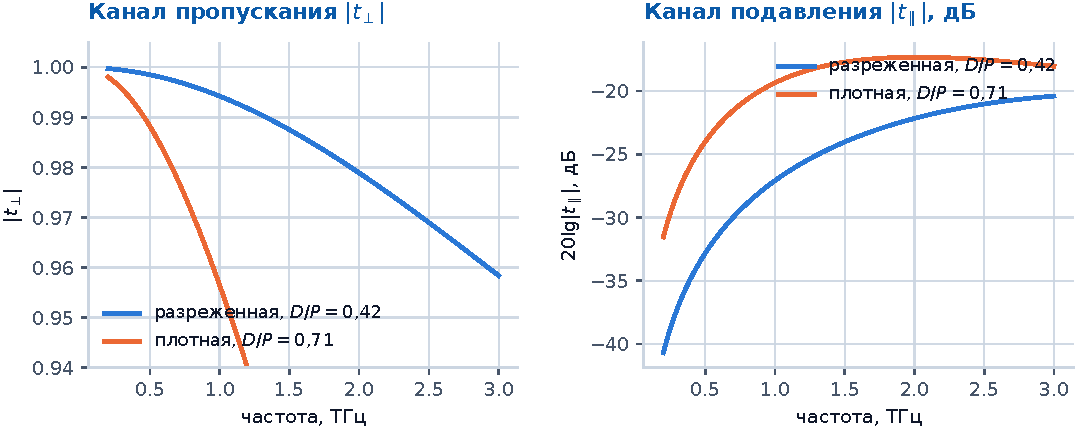
\includegraphics[width=\linewidth]{figures/fig02_transmission.pdf}
  \caption{Модельный расчёт $\tperp(\nu)$ и $\tpar(\nu)$ по формулам
  §§\ref{subsec:A1A2}--\ref{subsec:transmission} (без учёта конечной проводимости провода~---
  этот эффект вносится отдельным следующим слоем модели) для двух плотностей решётки на рабочей
  полосе частот.
  Канал пропускания уверенно держится у единицы независимо от плотности; канал подавления
  на порядки меньше и заметно чувствительнее к $D/P$.}
  \label{fig:blanco-spectrum}
\end{figure}

\begin{figure}[t]
  \centering
  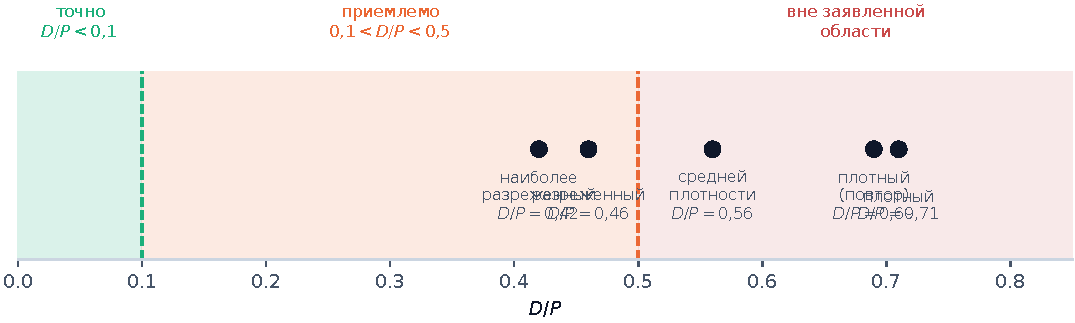
\includegraphics[width=\linewidth]{figures/fig02_validity_map.pdf}
  \caption{Карта применимости по параметру плотности $D/P$: узкая заявленная область точности,
  смягчённая граница приемлемости, область за пределами обеих и положение измеренных образцов
  (ключ~2.2). Условие $D/\lambda<0{,}2$ на этой оси не показано~--- оно выполнено для всех
  образцов с большим запасом на всей рабочей полосе частот (см. текст).}
  \label{fig:validity-map}
\end{figure}

% ---------------------------------------------------------------------
\subsection{Типичные ошибки этого параграфа}

\begin{enumerate}[leftmargin=1.6em,itemsep=0.25em]
  \item Спутать амплитудные коэффициенты $\tperp,\tpar$ с публикуемыми в первоисточнике
        мощностными $K_1,K_2$~--- та же ошибка на множитель два в децибелах, что и в
        §\ref{subsec:leakage}, только на входе модели.
  \item Проверять только $D/P<0{,}5$ и забыть про независимое условие $D/\lambda<0{,}2$~---
        оба должны выполняться одновременно.
  \item Считать резкой границей то, что на самом деле~--- постепенная потеря точности разложения
        по малому параметру; за формальной границей модель не обязана быть <<неверной>>, но
        доверие к ней требует отдельной проверки.
  \item Приписывать вещественную часть импеданса омическим потерям в проводе. В этой модели
        провод идеально проводящий; вещественная часть (недостижимая в нашей полосе частот)
        означает перекачку энергии в эванесцентные дифракционные порядки, а не нагрев.
  \item Забыть, что оба канала строятся из \emph{одних и тех же} чисел $A_1,A_2$~--- это не два
        независимых расчёта, а два разных сочетания одного и того же геометрического
        содержания.
\end{enumerate}

\clearpage
